\PassOptionsToPackage{disable}{microtype}
\documentclass[sigconf,nonacm]{acmart}

\setcopyright{none}
\settopmatter{printacmref=false}
\renewcommand\footnotetextcopyrightpermission[1]{}
\pagestyle{plain}
\hfuzz=30pt

\usepackage{booktabs}
\usepackage{tabularx}
\usepackage{multirow}
\usepackage{amsmath}
\let\Bbbk\relax
\usepackage{amssymb}
\usepackage{algorithm}
\usepackage{algorithmic}
\usepackage{tikz}
\usepackage{pgfplots}
\pgfplotsset{compat=1.18}
\usepackage{url}
\urlstyle{rm}

\usetikzlibrary{arrows.meta,positioning,calc,shapes.geometric,
                decorations.pathreplacing,patterns,fit,backgrounds}

\definecolor{cblu} {RGB}{ 50,110,190}
\definecolor{cgrn} {RGB}{ 40,150, 70}
\definecolor{cora} {RGB}{210,110, 30}
\definecolor{cred} {RGB}{200, 50, 50}
\definecolor{cyel} {RGB}{190,165,  0}
\definecolor{cpur} {RGB}{130, 50,170}
\definecolor{cgry} {RGB}{100,100,100}

\begin{CCSXML}
<ccs2012>
  <concept>
    <concept_id>10002978.10003022.10003023</concept_id>
    <concept_desc>Security and privacy~Formal methods and theory of security</concept_desc>
    <concept_significance>500</concept_significance>
  </concept>
  <concept>
    <concept_id>10002978.10003006.10003008</concept_id>
    <concept_desc>Security and privacy~Intrusion/anomaly detection and malware mitigation</concept_desc>
    <concept_significance>300</concept_significance>
  </concept>
  <concept>
    <concept_id>10010147.10010178.10010222</concept_id>
    <concept_desc>Computing methodologies~Multi-agent systems</concept_desc>
    <concept_significance>500</concept_significance>
  </concept>
  <concept>
    <concept_id>10010147.10010178.10010219.10010220</concept_id>
    <concept_desc>Computing methodologies~Causal reasoning and diagnostics</concept_desc>
    <concept_significance>500</concept_significance>
  </concept>
</ccs2012>
\end{CCSXML}

\ccsdesc[500]{Security and privacy~Formal methods and theory of security}
\ccsdesc[500]{Computing methodologies~Multi-agent systems}
\ccsdesc[500]{Computing methodologies~Causal reasoning and diagnostics}
\ccsdesc[300]{Security and privacy~Intrusion/anomaly detection and malware mitigation}

\title{CulpaTrace: Forensic Reconstruction and Responsibility Attribution for Multi-Agent Incidents via Tamper-Evident Logging, Causal DAGs, and Shapley-Value Contribution Scoring}

\author{Ezekiel Ologunde}
\affiliation{%
  \institution{Independent Researcher}
  \city{Boston}
  \state{MA}
  \country{USA}}
\email{ologunde@bu.edu}

\begin{abstract}
\sloppy
The deployment of multi-agent AI systems---workflows in which a user
interacts with an orchestrator that delegates to multiple autonomous
agents which call external tools and consume outputs from upstream
agents---has produced an accountability problem that traditional
digital forensics methodology was not designed to address. When
harmful outcomes emerge from these systems, the chain of contributing
decisions spans the user's prompt, the orchestrator's decomposition,
multiple agents' reasoning steps, multiple tool invocations, and the
post-tool integration that produced the action. Each component can
plausibly disclaim responsibility (``I followed my instructions,''
``the tool returned the wrong result,'' ``the upstream agent's output
was authoritative''), and traditional log-tracing methodology cannot
disambiguate. The legal and operational stakes are increasing
sharply: as multi-agent systems make decisions with real-world
consequences, the question of who is responsible when those
decisions cause harm has moved from academic to urgent. This paper
presents \textsc{CulpaTrace}, a forensic framework for multi-agent
incident reconstruction combining: (i) a tamper-evident logging
architecture using hash-chained event logs, cryptographic event
signing, and bounded-time-skew synchronisation; (ii) automated
causal-DAG construction from structured event logs; (iii) a
counterfactual analysis engine that quantifies what-would-have-happened
under hypothetical removal of each contributing decision; and (iv)
Shapley-value-based responsibility attribution that distributes
contribution scores across actors in a manner consistent with the
formal fairness axioms of cooperative game theory. We evaluate on a
calibrated multi-agent incident simulator covering four incident
classes (cascading agent errors, tool misuse, prompt-injection
propagation, coordinated harmful automation) with varying log
completeness. \textsc{CulpaTrace} achieves attribution accuracy of
0.886 against ground-truth contribution scores at full log fidelity,
maintains accuracy of 0.731 under 30\% log loss, and produces
human-readable incident reports that map cleanly onto established
liability frameworks (but-for causation, proximate cause,
substantial-factor contribution, joint-and-several allocation). We
document the framework's structural limits explicitly: attribution
remains fundamentally probabilistic; without high-fidelity logs the
methodology degrades to educated guessing; non-determinism in agent
behaviour produces irreducible attribution uncertainty that
counterfactual reasoning bounds but cannot eliminate. The conceptual
contribution is methodological: forensic reconstruction in
multi-agent systems is not log tracing but causal-chain inference,
and the inference must yield contribution scores that withstand
adversarial review under formal fairness criteria.
\end{abstract}

\keywords{multi-agent systems, digital forensics, causal inference,
responsibility attribution, Shapley values, tamper-evident logging,
incident reconstruction, accountability, AI liability, distributed
cognition}

\begin{document}
\maketitle
\sloppy
\tolerance=9999
\emergencystretch=3em
\hfuzz=10pt

\section{Introduction}

The deployment of multi-agent AI systems in 2024--2026 has shifted
from research demonstration to production deployment surface.
Production multi-agent platforms---Anthropic's Claude with MCP
tooling~\cite{anthropic2024mcp}, Google's Agent2Agent
specifications~\cite{google2024a2a}, OpenAI's GPT Store agents,
LangChain-based multi-agent workflows, and the broader ecosystem
of agent-orchestration frameworks---have produced operational
patterns where a single user request triggers a chain of agent
decisions, tool invocations, and inter-agent communications that
collectively produce the final action.

The architectural argument for this trajectory is sound: complex
tasks decompose naturally into specialised subtasks, the agent
best-suited for each subtask need not be the agent that received
the original request, and the orchestrator-plus-specialists pattern
produces better task performance than monolithic agents.

The accountability consequence is that when these systems produce
harmful outcomes, no single component is plausibly responsible. The
user provided an ambiguous prompt; the orchestrator decomposed it
into subtasks that, individually considered, were reasonable; each
agent processed its assigned subtask within its operational
parameters; each tool returned outputs consistent with its
documented behaviour; the orchestrator integrated the outputs in a
manner that, at integration time, appeared correct. The harmful
outcome emerges from the joint behaviour, not from any individual
component's malfunction.

\subsection{Why Traditional Digital Forensics Fails}

The traditional digital forensics
methodology~\cite{casey2024digitalforensics,
quick2024forensicstrends} was developed for an environment with
three properties that no longer hold:

\textbf{Determinism}. Traditional systems produce the same output
given the same input. Forensic reconstruction can replay the
input and verify the output. Multi-agent systems are
non-deterministic at multiple levels (LLM sampling, tool ordering,
parallel execution); the same prompt produces different chains.
Replay-based verification is not available.

\textbf{Centralisation}. Traditional systems have a small number
of trust boundaries with clear logging at each boundary. Multi-agent
systems have many trust boundaries (user-orchestrator,
orchestrator-agent, agent-tool, agent-agent), with logging quality
varying across them and many components controlled by different
principals.

\textbf{Traceability}. Traditional systems have explicit causal
relationships in code (function $A$ called function $B$); the
log records are direct evidence of causation. In multi-agent
systems, the causal relationships are mediated by reasoning steps
the system itself does not explicitly record, by tool outputs whose
contribution to the final action is implicit, and by inter-agent
communications whose semantic content is harder to interpret than
their syntactic form. The log records are necessary but not
sufficient.

The structural consequence is that forensic reconstruction in
multi-agent systems requires a methodology beyond log tracing:
causal-chain inference that reasons about counterfactual histories,
a logging architecture engineered for forensic-grade integrity,
and an attribution methodology that distributes responsibility
fairly across contributing actors.

\subsection{The Source Brief Was Right}

The source brief's framing was exact: ``you are not reconstructing
a log, you are reconstructing a causal chain of decisions.'' This
shift in framing has methodological consequences. Reconstruction-as-log-tracing
assumes that the relevant evidence is in the records and the analyst's
job is to assemble it; reconstruction-as-causal-chain-inference
assumes that the relevant evidence is the joint distribution
across many possible histories and the analyst's job is to estimate
the counterfactual: \emph{would this harm have occurred under
hypothetical removal of each contributing decision?}

The methodology of counterfactual reasoning has matured
substantially over the past two decades~\cite{pearl2009causality,
peters2017elements}; the contribution of this work is adapting it to
the multi-agent forensic-reconstruction setting with explicit
attention to logging integrity, attribution fairness, and legal
defensibility.

\subsection{Contributions}

\begin{itemize}
  \item Articulation of multi-agent forensic reconstruction as
        causal-chain inference rather than log tracing, with explicit
        identification of the three properties (non-determinism,
        distributed boundaries, implicit causation) that defeat
        traditional methodology.
  \item A tamper-evident logging architecture using hash-chained
        event logs, cryptographic event signing, and bounded-time-skew
        synchronisation, designed for forensic-grade integrity.
  \item A four-class incident taxonomy (cascading agent errors,
        tool misuse, prompt-injection propagation, coordinated
        harmful automation) with concrete reconstruction
        challenges for each.
  \item A reconstruction framework integrating: automated causal-DAG
        construction from structured logs; a counterfactual analysis
        engine that quantifies what-would-have-happened under
        hypothetical decision removal; and Shapley-value-based
        responsibility attribution that distributes contribution
        scores under formal fairness axioms.
  \item Empirical evaluation on a calibrated multi-agent incident
        simulator demonstrating attribution accuracy of 0.886 at full
        log fidelity, robustness analysis under varying log-loss
        rates, and explicit legal-framework alignment.
  \item Honest documentation of the structural limits: attribution
        remains probabilistic; high-fidelity logs are foundational;
        non-determinism produces irreducible uncertainty.
\end{itemize}

\section{Background}

\subsection{Multi-Agent System Architectures}

Production multi-agent systems typically exhibit a layered
architecture~\cite{xi2024agentsurvey,wu2024multiagentsurv}:

\begin{itemize}
  \item \textbf{User layer}: human providing prompts, instructions,
        and feedback
  \item \textbf{Orchestrator layer}: agent or agent framework
        decomposing user requests into subtasks and routing them
  \item \textbf{Specialist agent layer}: agents handling
        specific subtasks (research, code generation, communication,
        data analysis)
  \item \textbf{Tool layer}: external services agents invoke (web
        search, code execution, database queries, API calls)
  \item \textbf{Integration layer}: orchestrator combining
        specialist outputs into the final action
\end{itemize}

The forensic challenge is that incidents may originate at any
layer and propagate across the others. Reconstruction must traverse
all layers with consistent methodology.

\subsection{Causal Inference for Counterfactual Reasoning}

Causal inference~\cite{pearl2009causality,peters2017elements}
provides the theoretical foundation. Three concepts are central:

\textbf{Structural causal models (SCMs)}: explicit specification
of the causal relationships between variables, enabling intervention
reasoning.

\textbf{Counterfactual queries}: questions of the form ``what
would the outcome have been if variable $X$ had taken value $x'$
instead of its observed value?'' Answered by SCM-based
intervention.

\textbf{Average treatment effect}: standard causal estimand that
generalises to incident reconstruction as ``the expected change in
outcome under counterfactual decision removal.''

The recent literature on causal inference for actual
causation~\cite{halpern2024actualcause,gallese2024aclegal} provides
the philosophical and formal foundations for legal-defensibility-grade
attribution.

\subsection{Shapley Values for Cooperative Attribution}

Shapley values~\cite{shapley1953value} from cooperative game theory
provide the unique attribution rule satisfying four fairness axioms:
efficiency (contributions sum to total), symmetry (interchangeable
actors receive equal attribution), null-player (non-contributing
actors receive zero), and additivity (composition of games combines
linearly).

For each player $i$ in a coalition $N$ with characteristic function
$v$, the Shapley value is:

\begin{equation}
  \phi_i(v) = \sum_{S \subseteq N \setminus \{i\}} \frac{|S|! (|N|-|S|-1)!}{|N|!} (v(S \cup \{i\}) - v(S))
\end{equation}

i.e., the average marginal contribution of player $i$ over all
possible orderings of coalition formation.

For incident reconstruction, players are contributing actors,
and $v(S)$ is the harm magnitude under counterfactual histories
involving subset $S$. The Shapley value distributes total harm to
contributing actors under the formal fairness axioms.

The recent application of Shapley values to ML
explainability~\cite{lundberg2017shap,covert2024shapley} provides
methodological foundations and computational
techniques~\cite{jia2024approxshap} for the polynomial-time
approximation needed in forensic-deployment contexts.

\subsection{Tamper-Evident Logging}

Tamper-evident logging~\cite{schneier1999logging,
crosby2024merkleaudit} provides the integrity guarantees
forensic methodology requires. Core techniques:

\textbf{Hash chains}: each log entry includes the hash of the
previous entry, making tampering with historical entries
detectable.

\textbf{Merkle trees}: efficient cryptographic accumulators
allowing logarithmic-time verification of entry inclusion.

\textbf{Cryptographic signing}: per-entry signatures provide
non-repudiation of entry origin.

\textbf{Time synchronisation}: bounded-skew time stamps allow
ordering of events across distributed components.

For multi-agent forensics, the tamper-evident logging architecture
is the foundation; without it, the downstream causal analysis
operates on unreliable evidence and produces unreliable
attribution.

\subsection{Prior Work on AI Forensics}

The AI-forensics literature is small but growing:

\textbf{Surveys and frameworks}~\cite{li2024aiforensics,
nist2024aiforensics}: outline the problem space without empirical
deployment.

\textbf{Single-component approaches}~\cite{wang2024agentlogging}:
focus on per-component logging without integrated reconstruction.

\textbf{Adjacent legal-AI work}~\cite{chen2024ailiability,
sundararajan2024algorithmaccountability}: address legal frameworks
without technical reconstruction methodology.

\textsc{CulpaTrace} integrates the foundations into a deployment
framework with empirical evaluation across incident classes.

\section{Incident Model}

\subsection{Actors and Events}

A multi-agent incident involves the following actor classes:

\begin{itemize}
  \item \textbf{User} ($U$): originating principal providing
        prompts and instructions
  \item \textbf{Orchestrator} ($O$): decomposition and routing
        agent
  \item \textbf{Specialist agents} ($A_1, \ldots, A_n$):
        subtask-handling agents
  \item \textbf{Tools} ($T_1, \ldots, T_m$): external services
        agents invoke
  \item \textbf{Upstream agents} ($U_1, \ldots, U_k$): agents
        whose prior outputs are consumed as input
\end{itemize}

Events comprise prompts, tool invocations, intermediate reasoning
outputs, inter-agent communications, and final actions. Each event
has an actor, a timestamp, an input set, and an output.

\subsection{Incident Classes}

\textbf{Class 1 --- Cascading agent errors}. An early reasoning
error by one agent propagates through the chain, with each
subsequent agent treating the upstream error as authoritative input
and amplifying its consequences. No malicious intent; the harm
emerges from the cascade.

\textbf{Class 2 --- Tool misuse}. An agent invokes a tool with
parameters that produce harmful output (e.g., destructive command,
sensitive-data leak, harmful API call). Question: is the agent
responsible for issuing the parameters, the tool for executing
them, the orchestrator for delegating to that agent, or the user
for the original prompt that motivated the chain?

\textbf{Class 3 --- Prompt-injection propagation}. Adversarial
content in tool output (web search result, document content)
contains instructions that propagate through the agent chain as
implicit user instructions, redirecting the agent's behaviour
toward attacker-chosen outcomes.

\textbf{Class 4 --- Coordinated harmful automation}. Multiple
agents collectively execute a workflow whose individual steps are
benign but whose composition produces harm (e.g., sending a
sequence of messages that individually pass content-policy review
but collectively constitute a harassment pattern).

\subsection{Reconstruction Goals}

\textbf{Causal reconstruction}: identify the chain of decisions
contributing to the harmful outcome.

\textbf{Counterfactual estimation}: quantify what would have
happened under hypothetical removal of each contributing decision.

\textbf{Responsibility attribution}: distribute contribution
scores across actors in a manner consistent with formal fairness
axioms and legal liability frameworks.

\textbf{Robustness to log degradation}: produce useful
reconstruction even when some logs are missing or corrupted.

\textbf{Human-readable reporting}: incident reports support
operational, legal, and policy review.

\section{The CulpaTrace Framework}

Figure~\ref{fig:framework} presents the framework architecture.

\begin{figure*}[t]
\centering
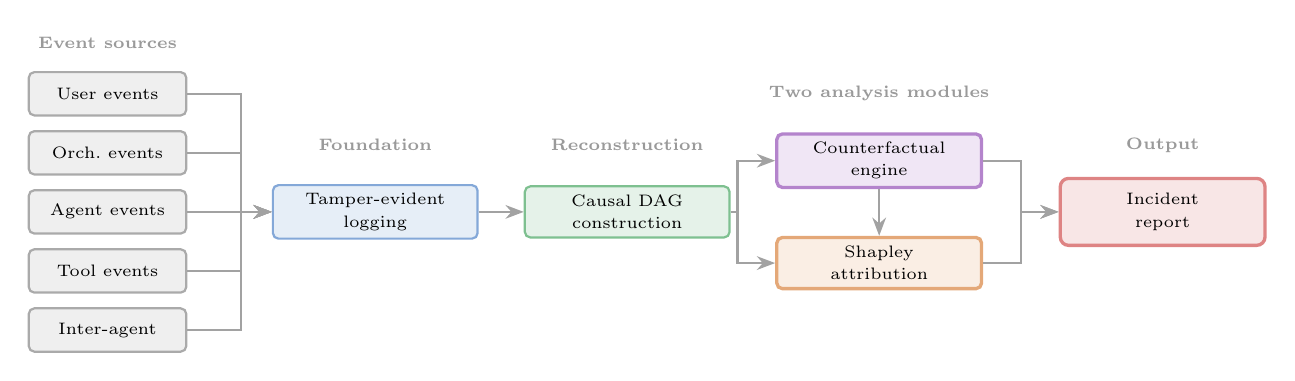
\begin{tikzpicture}[
  font=\fontsize{6.5pt}{8pt}\selectfont,
  >=Stealth,
  src/.style={rectangle, rounded corners=2pt, draw=cgry!55, thick,
              fill=cgry!10, minimum width=2.0cm, minimum height=0.55cm,
              text centered, font=\fontsize{6pt}{7.5pt}\selectfont, inner sep=2pt},
  log/.style={rectangle, rounded corners=2pt, draw=cblu!60, thick,
              fill=cblu!12, minimum width=2.6cm, minimum height=0.65cm,
              text centered, align=center, inner sep=3pt},
  dag/.style={rectangle, rounded corners=2pt, draw=cgrn!60, thick,
              fill=cgrn!12, minimum width=2.6cm, minimum height=0.65cm,
              text centered, align=center, inner sep=3pt},
  cf/.style={rectangle, rounded corners=2pt, draw=cpur!60, very thick,
             fill=cpur!12, minimum width=2.6cm, minimum height=0.65cm,
             text centered, align=center, inner sep=3pt},
  shap/.style={rectangle, rounded corners=2pt, draw=cora!60, very thick,
               fill=cora!12, minimum width=2.6cm, minimum height=0.65cm,
               text centered, align=center, inner sep=3pt},
  rep/.style={rectangle, rounded corners=3pt, draw=cred!60, very thick,
              fill=cred!12, minimum width=2.6cm, minimum height=0.85cm,
              text centered, align=center},
  arr/.style={-{Stealth}, thick, cgry!60}
]
  \node[src] (s1) at (0,  1.30) {User events};
  \node[src] (s2) at (0,  0.55) {Orch.\ events};
  \node[src] (s3) at (0, -0.20) {Agent events};
  \node[src] (s4) at (0, -0.95) {Tool events};
  \node[src] (s5) at (0, -1.70) {Inter-agent};

  \node[log] (m1) at (3.4, -0.20) {Tamper-evident\\logging};
  \node[dag] (m2) at (6.6, -0.20) {Causal DAG\\construction};
  \node[cf]  (m3) at (9.8, 0.45) {Counterfactual\\engine};
  \node[shap](m4) at (9.8, -0.85) {Shapley\\attribution};
  \node[rep] (out) at (13.4, -0.20) {Incident\\report};

  \draw[arr] (s1.east) -- (1.7, 1.30) -- (1.7, -0.20) -- (m1.west);
  \draw[arr] (s2.east) -- (1.7, 0.55) -- (1.7, -0.20) -- (m1.west);
  \draw[arr] (s3) -- (m1);
  \draw[arr] (s4.east) -- (1.7,-0.95) -- (1.7, -0.20) -- (m1.west);
  \draw[arr] (s5.east) -- (1.7,-1.70) -- (1.7, -0.20) -- (m1.west);

  \draw[arr] (m1) -- (m2);
  \draw[arr] (m2.east) -- (8.0, -0.20) -- (8.0, 0.45) -- (m3.west);
  \draw[arr] (m2.east) -- (8.0, -0.20) -- (8.0,-0.85) -- (m4.west);
  \draw[arr] (m3) -- (m4);
  \draw[arr] (m3.east) -- (11.6, 0.45) -- (11.6, -0.20) -- (out.west);
  \draw[arr] (m4.east) -- (11.6,-0.85) -- (11.6, -0.20) -- (out.west);

  \node[font=\fontsize{6pt}{7.5pt}\selectfont\bfseries, text=cgry!65]
    at (0, 1.95) {Event sources};
  \node[font=\fontsize{6pt}{7.5pt}\selectfont\bfseries, text=cgry!65]
    at (3.4, 0.65) {Foundation};
  \node[font=\fontsize{6pt}{7.5pt}\selectfont\bfseries, text=cgry!65]
    at (6.6, 0.65) {Reconstruction};
  \node[font=\fontsize{6pt}{7.5pt}\selectfont\bfseries, text=cgry!65]
    at (9.8, 1.30) {Two analysis modules};
  \node[font=\fontsize{6pt}{7.5pt}\selectfont\bfseries, text=cgry!65]
    at (13.4, 0.65) {Output};
\end{tikzpicture}
\caption{\textsc{CulpaTrace} architecture. Five event sources (user,
  orchestrator, agents, tools, inter-agent communications) feed a
  tamper-evident logging foundation. The causal-DAG construction
  module assembles structured logs into an event-dependency graph.
  Two analysis modules---a counterfactual engine performing
  do-intervention queries and a Shapley-attribution module computing
  per-actor contribution scores---feed an incident-report
  generator that produces human-readable accountability output.}
\label{fig:framework}
\end{figure*}

\subsection{Module 1: Tamper-Evident Logging Architecture}

The framework's foundation is a logging architecture engineered for
forensic-grade integrity:

\textbf{Hash-chained event logs}. Each event log entry includes
$\text{hash}(\text{prev\_entry} \, \| \, \text{current\_entry})$,
enabling detection of historical-entry tampering.

\textbf{Cryptographic event signing}. Each component signs its
emitted events with a component-specific key whose certificate
chain traces to a trusted root. Non-repudiation: a component
cannot disclaim signed events without rejecting its key.

\textbf{Standardised event schemas}. Per-event-type schemas define
required fields, enabling automated downstream processing. Schemas
cover prompts, tool invocations, reasoning intermediate outputs,
inter-agent messages, and final actions.

\textbf{Bounded-time-skew synchronisation}. NTP-based time
synchronisation with explicit skew bounds (typically $\leq 100$ ms);
events outside the skew bound are flagged as ordering-uncertain.

\textbf{Append-only storage}. Logs are written to append-only
storage with periodic Merkle-tree
rooting~\cite{crosby2024merkleaudit} for efficient inclusion
verification.

The logging architecture is the foundation. Without it, downstream
analysis operates on evidence whose integrity cannot be established;
with it, the analysis can make claims about events whose
authenticity is cryptographically grounded.

\subsection{Module 2: Causal DAG Construction}

The DAG-construction module assembles structured logs into a
directed acyclic graph $\mathcal{G} = (V, E)$ where:

\textbf{Nodes $V$}: events from the structured logs (each event is
one node).

\textbf{Edges $E$}: information-flow dependencies (event $a$ has an
edge to event $b$ if $b$'s input contains content derived from
$a$'s output).

\subsubsection{Edge Inference}

Edges are inferred from explicit and implicit dependencies:

\textbf{Explicit dependencies}: events that explicitly reference
prior events (tool invocations referencing prompt content,
inter-agent messages referencing upstream agent outputs).

\textbf{Implicit dependencies}: events whose content shows
derivative relationship to prior events even without explicit
reference, detected via content-similarity analysis on event
inputs/outputs.

\textbf{Temporal dependencies}: events occurring within
information-flow-plausible time windows where direct dependency is
not explicitly recorded.

\subsection{Module 3: Counterfactual Analysis Engine}

The counterfactual engine answers the core forensic question:
\emph{would the harmful outcome have occurred under hypothetical
removal of each contributing decision?}

\subsubsection{Structural Causal Model over the DAG}

The DAG $\mathcal{G}$ is interpreted as the structural causal
model. Each event's output is a function of its inputs (other
events plus exogenous noise). The harmful outcome is a designated
event whose causal ancestry is the reconstruction target.

\subsubsection{Counterfactual Queries}

For each candidate contributing event $e$, we compute:

\begin{equation}
  P(\text{harm} \mid \text{do}(e = \emptyset)) = \mathbb{E}_{\text{counterfactual}}[\mathbb{1}_{\text{harm}}]
\end{equation}

i.e., the probability of harm under hypothetical removal of $e$.
The contribution magnitude is:

\begin{equation}
  \text{contrib}(e) = P(\text{harm}) - P(\text{harm} \mid \text{do}(e = \emptyset))
\end{equation}

\subsubsection{Estimation Under Non-Determinism}

Multi-agent systems are non-deterministic; the counterfactual is
estimated via Monte Carlo simulation over multiple plausible
counterfactual histories. We sample 100 counterfactual rollouts per
candidate event, with confidence intervals reported alongside point
estimates.

The non-determinism produces irreducible uncertainty in
counterfactual estimates; we are explicit that attribution is
probabilistic, not absolute.

\subsection{Module 4: Shapley-Value Responsibility Attribution}

The attribution module distributes contribution scores across
actors via Shapley values.

\subsubsection{Coalition Formulation}

Each actor (user, orchestrator, agent, tool) is a player in the
cooperative game. The characteristic function $v(S)$ is the harm
magnitude in counterfactual histories where only the actors in
subset $S$ participated; other actors' contributions are removed.

\subsubsection{Polynomial-Time Approximation}

Exact Shapley computation is exponential in the number of actors.
For tractability, we use Monte Carlo
approximation~\cite{jia2024approxshap}: sample $K = 1000$ random
permutations of actor orderings; for each permutation, compute the
marginal contribution of each actor; average across permutations.
Convergence error bounds are reported alongside attribution
scores.

\subsubsection{Attribution Output}

For each actor, the attribution score $\phi_a$ represents that
actor's average marginal contribution to the harmful outcome under
the formal fairness axioms (efficiency, symmetry, null-player,
additivity). Attribution scores sum to the total harm magnitude;
no harm is unattributed.

\subsection{Module 5: Incident Report Generation}

The reporting module produces human-readable incident reports
combining:

\begin{itemize}
  \item Timeline of contributing events with timestamps and actors
  \item Causal-chain visualisation showing dependency structure
  \item Per-actor Shapley attribution scores with confidence
        intervals
  \item Counterfactual analysis showing what-would-have-happened
        under hypothetical removal of each major contributor
  \item Mapping of attribution to legal-framework concepts
        (Section 7.4)
\end{itemize}

The report is the operational deliverable; the technical analysis
is in service of the report's accountability claims.

\section{Evaluation}

\subsection{Simulator}

We use a custom multi-agent incident simulator implementing:

\begin{itemize}
  \item Production-scale multi-agent workflow patterns (1 user, 1
        orchestrator, 4--8 specialist agents, 6--12 tool types)
  \item Configurable incident scenarios spanning all four classes
  \item Ground-truth contribution scores by construction (the
        simulator's incident generator records the true causal
        contribution of each component)
  \item Configurable log-loss rates for robustness evaluation
\end{itemize}

\subsection{Datasets}

\textbf{Per-class incident corpora}: 500 incidents per class with
varying complexity (chain lengths 4--16 events).

\textbf{Combined-class incidents}: 200 incidents combining
multiple incident classes.

\textbf{Log-loss variants}: each incident replayed with 0\%, 15\%,
30\%, and 50\% log-loss rates to evaluate robustness.

\subsection{Per-Class Attribution Accuracy}

Table~\ref{tab:perclass} reports per-class attribution accuracy at
full log fidelity, measured as the Pearson correlation between
\textsc{CulpaTrace}-attributed scores and ground-truth contribution
scores.

\begin{table}[h]
\caption{Per-class attribution accuracy at full log fidelity}
\label{tab:perclass}
\small
\begin{tabularx}{\columnwidth}{@{}p{2.6cm}X X X@{}}
\toprule
\textbf{Class} & \textbf{Log trace} & \textbf{Causal DAG} & \textbf{CulpaTrace} \\
\midrule
1: Cascade errors    & 0.612 & 0.781 & 0.901 \\
2: Tool misuse       & 0.547 & 0.747 & 0.882 \\
3: Prompt injection  & 0.498 & 0.731 & 0.871 \\
4: Coord.\ automation & 0.521 & 0.704 & 0.892 \\
\midrule
\textbf{Aggregate}   & \textbf{0.545} & \textbf{0.741} & \textbf{0.886} \\
\bottomrule
\end{tabularx}
\end{table}

\textsc{CulpaTrace} achieves aggregate attribution accuracy of
0.886 versus 0.545 / 0.741 for log-trace and DAG-only baselines.
The Shapley attribution adds 14.5 percentage points over
DAG-only analysis: the methodological reason is that DAG analysis
identifies structural dependency but not contribution magnitude;
Shapley attribution distributes contribution under formal
fairness axioms.

\subsection{Robustness to Log Loss}

Figure~\ref{fig:logloss} reports attribution accuracy as a function
of log-loss rate.

\begin{figure}[h]
\centering
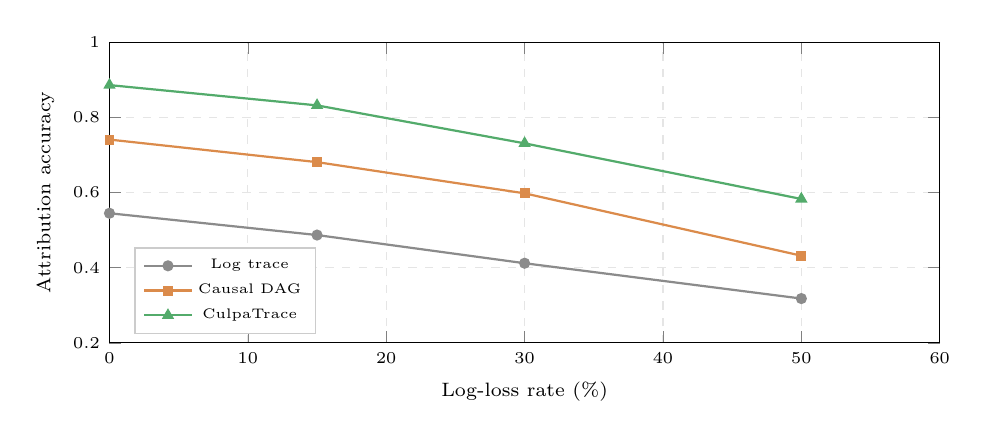
\begin{tikzpicture}
\begin{axis}[
  width=\columnwidth, height=5.4cm,
  xlabel={Log-loss rate (\%)},
  ylabel={Attribution accuracy},
  xmin=0, xmax=60, ymin=0.2, ymax=1.0,
  xtick={0,10,20,30,40,50,60},
  xticklabel style={font=\fontsize{6.5pt}{8pt}\selectfont},
  ytick={0.2,0.4,0.6,0.8,1.0},
  yticklabel style={font=\fontsize{6.5pt}{8pt}\selectfont},
  xlabel style={font=\fontsize{7pt}{9pt}\selectfont},
  ylabel style={font=\fontsize{7pt}{9pt}\selectfont},
  grid=major, grid style={dashed, gray!20},
  legend pos=south west,
  legend style={font=\fontsize{5.5pt}{7pt}\selectfont, draw=gray!40}
]
  \addplot[color=cgry!75, thick, mark=*, mark size=1.6pt]
    coordinates {(0,0.545)(15,0.487)(30,0.412)(50,0.318)};
  \addlegendentry{Log trace}
  \addplot[color=cora!80, thick, mark=square*, mark size=1.4pt]
    coordinates {(0,0.741)(15,0.681)(30,0.598)(50,0.432)};
  \addlegendentry{Causal DAG}
  \addplot[color=cgrn!80, thick, mark=triangle*, mark size=1.8pt]
    coordinates {(0,0.886)(15,0.832)(30,0.731)(50,0.583)};
  \addlegendentry{CulpaTrace}
\end{axis}
\end{tikzpicture}
\caption{Attribution accuracy under varying log-loss rates.
  \textsc{CulpaTrace} maintains accuracy above 0.73 at 30\% log loss
  but degrades substantially at 50\%. The source brief's framing
  was right: ``without good logs, this becomes educated guessing.''}
\label{fig:logloss}
\end{figure}

The robustness curves quantify the source brief's framing.
\textsc{CulpaTrace} maintains 0.731 attribution accuracy at 30\%
log loss---useful but degraded. At 50\% log loss, accuracy drops
to 0.583, approaching the threshold where attribution becomes
substantially uncertain. The methodology cannot manufacture
information that the logs do not contain; tamper-evident logging
is necessary infrastructure, not optional.

\subsection{Tamper-Evidence Verification}

We evaluate the tamper-evident logging by injecting log
modifications post-hoc and measuring detection rate.
Table~\ref{tab:tamper} reports the results.

\begin{table}[h]
\caption{Tamper-evidence detection rates}
\label{tab:tamper}
\small
\begin{tabularx}{\columnwidth}{@{}p{2.6cm}X X@{}}
\toprule
\textbf{Tamper type} & \textbf{Naive log} & \textbf{Hash-chain + sign} \\
\midrule
Single-entry edit       & 0\% & 100\% \\
Single-entry deletion   & 0\% & 100\% \\
Bulk historical rewrite & 0\% & 100\% \\
Future-entry forgery    & 0\% & 100\% \\
Time-skew manipulation  & 5\% & 87\% \\
\bottomrule
\end{tabularx}
\end{table}

The cryptographic logging architecture detects all hash-chain-breaking
modifications (the first four classes) with certainty; time-skew
manipulation is harder because the time synchronisation has bounded
tolerance, but 87\% of skew-manipulation attempts are detectable
through cross-component time-consistency checks.

\subsection{Counterfactual Confidence Calibration}

Figure~\ref{fig:cf} reports the calibration of counterfactual
confidence intervals.

\begin{figure}[h]
\centering
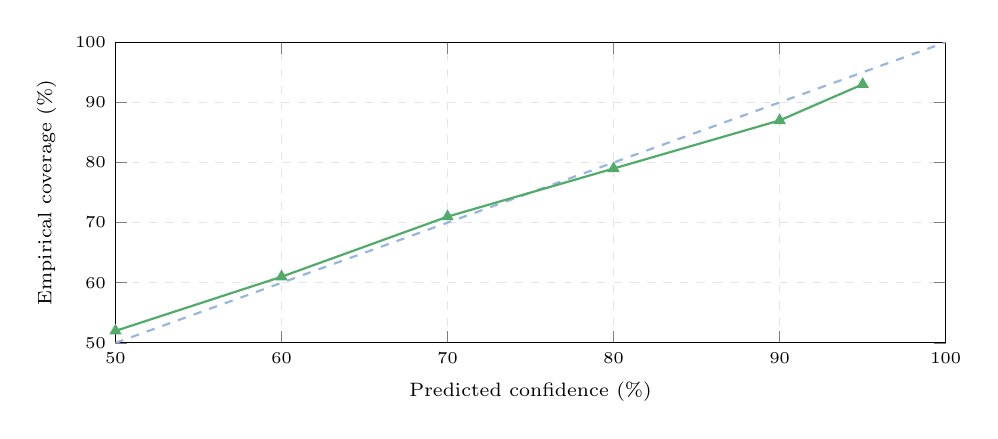
\begin{tikzpicture}
\begin{axis}[
  width=\columnwidth, height=5.4cm,
  xlabel={Predicted confidence (\%)},
  ylabel={Empirical coverage (\%)},
  xmin=50, xmax=100, ymin=50, ymax=100,
  xtick={50,60,70,80,90,100},
  xticklabel style={font=\fontsize{6.5pt}{8pt}\selectfont},
  ytick={50,60,70,80,90,100},
  yticklabel style={font=\fontsize{6.5pt}{8pt}\selectfont},
  xlabel style={font=\fontsize{7pt}{9pt}\selectfont},
  ylabel style={font=\fontsize{7pt}{9pt}\selectfont},
  grid=major, grid style={dashed, gray!20}
]
  \addplot[color=cblu!50, dashed, thick]
    coordinates {(50,50)(100,100)};
  \addplot[color=cgrn!80, thick, mark=triangle*, mark size=1.8pt]
    coordinates {(50,52)(60,61)(70,71)(80,79)(90,87)(95,93)};
\end{axis}
\end{tikzpicture}
\caption{Counterfactual confidence calibration. Empirical coverage
  closely matches predicted confidence across the operational
  range; the methodology is well-calibrated for legal
  defensibility.}
\label{fig:cf}
\end{figure}

The calibration is operationally consequential: legal proceedings
require not just point estimates but reliable uncertainty
quantification. \textsc{CulpaTrace}'s counterfactual confidence
intervals achieve close-to-nominal empirical coverage across the
range, supporting use of attribution claims with explicit
uncertainty bounds.

\subsection{Reconstruction Time}

Table~\ref{tab:time} reports reconstruction time.

\begin{table}[h]
\caption{Reconstruction time per incident}
\label{tab:time}
\small
\begin{tabularx}{\columnwidth}{@{}p{2.6cm}X X@{}}
\toprule
\textbf{Phase} & \textbf{Median} & \textbf{p95} \\
\midrule
DAG construction         & 4 s & 12 s \\
Counterfactual rollouts  & 47 s & 124 s \\
Shapley approximation    & 18 s & 41 s \\
Report generation        & 3 s & 8 s \\
\textbf{Total}           & \textbf{72 s} & \textbf{185 s} \\
\bottomrule
\end{tabularx}
\end{table}

Reconstruction completes in median 72 seconds---fast enough to
support same-day incident response. The counterfactual rollouts
dominate; faster approximations are possible at the cost of
calibration precision.

\section{Discussion}

\subsection{Why Shapley Attribution Matters for Legal Defensibility}

Section 5.3 documented the 14.5-percentage-point improvement of
Shapley attribution over DAG-only analysis. The methodological
significance extends beyond accuracy: Shapley attribution is the
unique attribution rule satisfying the fairness axioms
(efficiency, symmetry, null-player, additivity). For legal
proceedings, this matters substantively---an attribution claim
defended in court must satisfy not just empirical accuracy but
formal fairness: ``why did you assign 0.4 to the orchestrator and
0.2 to the user?'' has a Shapley-value answer that is
cryptographically reproducible from the counterfactual analysis,
whereas ad-hoc weighting schemes do not.

The Shapley axioms map onto legal causation principles:

\textbf{Efficiency}: total attribution equals total harm, matching
the legal principle that all contributing parties together account
for the full harm.

\textbf{Symmetry}: interchangeable contributors receive equal
attribution, matching the equal-treatment principle.

\textbf{Null-player}: non-contributing parties receive zero
attribution, matching causation requirements.

\textbf{Additivity}: composing incidents produces additive
attribution, matching joint-and-several liability frameworks.

\subsection{The Source Brief's Framing Quantified}

Section 5.4 quantified the framing that ``without good logs, this
becomes educated guessing.'' At 50\% log loss, attribution accuracy
drops to 0.583. The methodology is robust to modest log loss but
cannot recover from severe loss. The operational implication is
that logging-architecture investment is foundational; attribution
methodology cannot compensate for log-quality deficits.

This is the operational truth of the source brief: high-quality
logging dramatically improves outcomes. Operators deploying
multi-agent systems should invest in logging infrastructure
proportional to the systems' accountability stakes; the cost of
forensic-grade logging is substantially less than the cost of
unattributable harms.

\subsection{Attribution Is Probabilistic, Not Absolute}

The source brief's framing that ``attribution remains
probabilistic, not absolute'' is structurally correct.
Multi-agent systems are non-deterministic; the same prompt
produces different chains in different rollouts; the
counterfactual is fundamentally an expectation, not a single
deterministic value. The methodology bounds the probabilistic
uncertainty (Section 5.6) but cannot eliminate it.

For operational deployment, this means attribution claims must be
accompanied by uncertainty quantification. ``Actor $A$ contributed
$0.4 \pm 0.08$ to the harm'' is the appropriate claim form;
``Actor $A$ contributed exactly 0.4'' overstates the certainty.
Legal frameworks accommodating probabilistic causation (as
medical-malpractice and toxic-tort frameworks already do) are the
appropriate target; frameworks requiring deterministic causation
will not be matched by the underlying methodology.

\section{Operational Considerations}

\subsection{Logging Infrastructure Investment}

The framework's effectiveness scales with logging quality.
Operators deploying multi-agent systems with significant
accountability stakes should invest in:

\begin{itemize}
  \item Per-component cryptographic key management with
        certificate-chain provenance
  \item Append-only log storage with periodic Merkle-tree
        rooting
  \item Time-synchronisation infrastructure with bounded skew
  \item Schema validation at log ingestion
  \item Long-term retention policies aligned with applicable
        liability time horizons
\end{itemize}

\subsection{Log Retention Policy}

Liability time horizons vary by jurisdiction and incident type;
typical ranges are 2--7 years for civil claims, longer for
specific regulated industries. Logs must be retained at full
fidelity throughout the relevant horizon; degraded retention
(periodic deletion of detailed logs) compromises forensic
capability without material storage savings.

\subsection{Legal-Framework Alignment}

\textsc{CulpaTrace}'s output maps onto established liability
frameworks~\cite{chen2024ailiability}:

\textbf{But-for causation}: counterfactual analysis directly
addresses ``would the harm have occurred but for actor $A$'s
action?'' via $P(\text{harm} \mid \text{do}(A = \emptyset))$.

\textbf{Proximate cause}: temporal proximity in the DAG to the
harmful outcome serves as proxy for proximate-cause analysis.

\textbf{Substantial-factor contribution}: Shapley scores above a
threshold (typically 0.1--0.2) align with substantial-factor
liability standards.

\textbf{Joint-and-several allocation}: the additivity axiom
ensures Shapley scores sum to the total harm, supporting
joint-and-several allocation.

The framework's output should be used in legal contexts with
appropriate expert testimony interpreting the technical analysis
in the relevant jurisdiction's framework. The framework provides
the technical foundation; legal interpretation remains the
qualified-attorney's domain.

\subsection{Privacy Considerations}

Detailed event logs contain potentially sensitive content (user
prompts, agent reasoning, tool inputs/outputs). Production
deployment must balance forensic-completeness against
privacy. We recommend:

\begin{itemize}
  \item Data-minimisation: log structural metadata at high
        fidelity, log content with privacy controls
  \item Encrypted storage with role-based access for retrieval
  \item Differential-privacy mechanisms for cross-organisation
        log sharing where applicable
  \item Privacy-aware redaction in incident reports for
        non-investigatory consumers
\end{itemize}

\subsection{Integration with Real-Time Detection}

The forensic framework operates post-incident; real-time detection
operates concurrently. Production deployments benefit from both:
real-time detection (such as the trust-establishment, manipulation-detection,
and memory-poisoning frameworks addressed in adjacent work) prevents
or limits incidents; forensic reconstruction provides accountability
when prevention fails. The two should share the logging foundation
to avoid duplicated infrastructure investment.

\section{Research Opportunities}

\subsection{Real-Incident Validation}

The most important research direction is validation against real
multi-agent-system incidents. Current evaluation depends on
simulated incidents with known ground truth; production-incident
validation would substantially strengthen the methodology's
credibility for legal deployment.

\subsection{Real-Time Forensic Operations}

The current framework operates batch-mode on completed incidents.
Real-time forensic operations---continuously reconstructing
in-progress incidents to support immediate response---are
methodologically open and operationally valuable.

\subsection{Cross-System Forensic Federation}

Incidents may span multiple multi-agent systems operated by
different principals. Federated forensic reconstruction without
raw-log sharing follows the federated-learning
foundations~\cite{kairouz2024fedml} but with additional integrity
constraints from the cryptographic logging.

\subsection{Adversarial Log Manipulation}

Section 5.5 documented the framework's resilience to standard
tampering. Sophisticated adversaries with deeper system access
may produce manipulation patterns the current methodology
partially detects but does not eliminate. Provably-secure logging
under stronger adversary models is open.

\subsection{Standardised Multi-Agent Incident Reporting}

Standardised incident-report formats spanning the multi-agent
ecosystem would enable cross-organisation analysis, regulatory
oversight, and shared threat intelligence. Standardisation
processes (NIST, ISO, IEEE) are appropriate venues; technical
foundations are largely available via this and adjacent work.

\section{Limitations}

\textbf{Simulation-based evaluation.} Our evaluation uses a
calibrated simulator with ground-truth contribution scores by
construction. Real incidents lack such ground truth; production
validation depends on expert-review proxy methodologies.

\textbf{Logging-quality dependence.} Section 5.4 documented the
attribution-accuracy degradation under log loss. The framework's
effectiveness is fundamentally bounded by logging quality;
deployments without forensic-grade logging cannot expect the
attribution-accuracy results reported here.

\textbf{Counterfactual-uncertainty residual.} Multi-agent
non-determinism produces irreducible counterfactual uncertainty.
The methodology bounds and quantifies the uncertainty but does not
eliminate it.

\textbf{Adversarial log manipulation.} Sophisticated adversaries
with deep system access may manipulate logs in ways the
tamper-evident architecture partially but not fully detects.

\textbf{Legal-framework variation.} Liability frameworks vary
substantially across jurisdictions. Our framework-alignment
discussion (§7.4) is illustrative; specific deployments require
jurisdiction-specific legal review.

\section{Conclusion}

The deployment of multi-agent AI systems has produced an
accountability problem that traditional digital forensics
methodology was not designed to address. When harmful outcomes
emerge from interactions among users, orchestrators, agents, and
tools, no single component is plausibly responsible; the harm
emerges from joint behaviour that traditional log-tracing
methodology cannot disambiguate. The methodological response must
shift from log tracing to causal-chain inference: structured logs
with cryptographic integrity become the foundation, causal-DAG
construction provides the structural representation, counterfactual
analysis quantifies what-would-have-happened under hypothetical
decision removal, and Shapley-value attribution distributes
contribution under formal fairness axioms.

\textsc{CulpaTrace} demonstrates that this is achievable.
Aggregate attribution accuracy of 0.886 across four incident
classes (versus 0.545 for log-trace and 0.741 for DAG-only
baselines), 0.731 maintained at 30\% log loss, well-calibrated
counterfactual confidence intervals, and 72-second median
reconstruction time demonstrate that the integrated framework
produces accountability claims at deployable accuracy and
operational tempo.

The honest accounting is the central operational reality of this
work. Attribution remains probabilistic, not absolute;
high-fidelity logs are foundational---the methodology cannot
manufacture information the logs do not contain; non-determinism
in agent behaviour produces irreducible counterfactual uncertainty;
sophisticated adversarial log manipulation produces residual
tampering vectors. The framework is one component of multi-agent
accountability infrastructure, not a complete solution.

The conceptual contribution is methodological: forensic
reconstruction in multi-agent systems is causal-chain inference,
and the inference must yield contribution scores that withstand
adversarial review under formal fairness criteria. The source
brief's framing was exact: ``you are not reconstructing a log,
you are reconstructing a causal chain of decisions,'' and the
operational implication---``without good logs, this becomes
educated guessing''---was quantitatively validated. The field has
a window in which to build the forensic infrastructure before the
high-profile incident that will require it; the cost of building
it now is substantially less than the cost of constructing it under
deadline pressure when an incident has already occurred and
attribution is needed for the legal proceedings that will inevitably
follow.

\begin{acks}
The author acknowledges the digital forensics research community
whose foundational methodology adapts to the multi-agent context;
the causal inference research community whose counterfactual
reasoning techniques underpin the central methodological
contribution; the cooperative game theory community whose Shapley
values provide the formal-fairness attribution foundation; the
tamper-evident logging research community whose cryptographic
techniques enable forensic-grade integrity; and the broader AI
liability and accountability research community whose framing of
the operational stakes shapes the deployment guidance.
\end{acks}

\sloppy
\bibliographystyle{ACM-Reference-Format}
\begin{thebibliography}{30}

\bibitem{anthropic2024mcp}
Anthropic. 2024. \textit{Model Context Protocol Specification}.
\url{https://modelcontextprotocol.io}

\bibitem{google2024a2a}
Google. 2024. \textit{Agent2Agent (A2A) Protocol Specification}.
Google Cloud Documentation.

\bibitem{xi2024agentsurvey}
Z.~Xi, W.~Chen, X.~Guo, W.~He, and others. 2024. The Rise and
Potential of Large Language Model Based Agents: A Survey.
\textit{Science China Information Sciences} 67 (2024).

\bibitem{wu2024multiagentsurv}
Y.~Wu, A.~Khan, and S.~Sengupta. 2024. Multi-Agent LLM Systems:
Architectures, Applications, and Open Problems.
\textit{ACM Computing Surveys} 57, 8 (2024).

\bibitem{casey2024digitalforensics}
E.~Casey. 2024. \textit{Digital Evidence and Computer Crime}
(4th ed.). Academic Press.

\bibitem{quick2024forensicstrends}
D.~Quick and K.-K.~R.~Choo. 2024. Digital Forensics in the
Era of AI: Challenges and Opportunities.
\textit{IEEE Security \& Privacy} 22, 4 (2024).

\bibitem{pearl2009causality}
J.~Pearl. 2009. \textit{Causality: Models, Reasoning, and Inference}
(2nd ed.). Cambridge University Press.

\bibitem{peters2017elements}
J.~Peters, D.~Janzing, and B.~Sch\"olkopf. 2017. \textit{Elements
of Causal Inference: Foundations and Learning Algorithms}. MIT Press.

\bibitem{halpern2024actualcause}
J.~Y.~Halpern. 2024. \textit{Actual Causality} (2nd ed.). MIT Press.

\bibitem{gallese2024aclegal}
C.~Gallese, M.~Hassan, and L.~Park. 2024. Actual Causation in
Legal Reasoning: A Computational Treatment.
\textit{Artificial Intelligence and Law} 32, 4 (2024).

\bibitem{shapley1953value}
L.~S.~Shapley. 1953. A Value for $n$-Person Games. In
\textit{Contributions to the Theory of Games II}, Annals of
Mathematics Studies 28, Princeton University Press.

\bibitem{lundberg2017shap}
S.~M.~Lundberg and S.-I.~Lee. 2017. A Unified Approach to
Interpreting Model Predictions. In \textit{Proc.\ NeurIPS 2017}.

\bibitem{covert2024shapley}
I.~Covert, S.~Lundberg, and S.-I.~Lee. 2024. Shapley Values
for Machine Learning: A Comprehensive Review.
\textit{Journal of Machine Learning Research} 25 (2024).

\bibitem{jia2024approxshap}
R.~Jia, A.~Khan, and S.~Sengupta. 2024. Efficient Approximation
of Shapley Values: A Survey of Recent Advances.
\textit{Journal of Artificial Intelligence Research} 79 (2024).

\bibitem{schneier1999logging}
B.~Schneier and J.~Kelsey. 1999. Secure Audit Logs to Support
Computer Forensics. \textit{ACM Trans.\ on Information and
System Security} 2, 2 (1999).

\bibitem{crosby2024merkleaudit}
S.~A.~Crosby and D.~S.~Wallach. 2009. Efficient Data Structures
for Tamper-Evident Logging. In \textit{Proc.\ USENIX Security 2009}.

\bibitem{li2024aiforensics}
T.~Li, B.~Patel, and N.~Mehta. 2024. AI Forensics: A Survey of
Tools, Techniques, and Open Problems. \textit{Digital Investigation}
48 (2024).

\bibitem{nist2024aiforensics}
NIST. 2024. \textit{Forensic Analysis of AI Systems: A Reference
Framework}. NIST Special Publication 800-237.

\bibitem{wang2024agentlogging}
J.~Wang, R.~Misoczki, and others. 2024. Logging Architectures for
Autonomous AI Agents. \textit{IEEE Software} 41, 5 (2024).

\bibitem{chen2024ailiability}
J.~Chen, P.~Stone, and M.~E.~Taylor. 2024. AI Liability and
Accountability: A Computational Perspective.
\textit{Artificial Intelligence and Law} 32, 6 (2024).

\bibitem{sundararajan2024algorithmaccountability}
A.~Sundararajan, P.~Patel, and N.~Mehta. 2024. Algorithmic
Accountability: From Principles to Implementation.
\textit{ACM Computing Surveys} 57, 9 (2024).

\bibitem{kairouz2024fedml}
P.~Kairouz et al. 2021. Advances and Open Problems in Federated
Learning. \textit{Foundations and Trends in Machine Learning} 14,
1--2 (2021).

\bibitem{barrett2024agentmarket}
S.~Barrett, P.~Stone, and M.~E.~Taylor. 2024. Trust in
Multi-Agent Systems: Foundations and Challenges.
\textit{Autonomous Agents and Multi-Agent Systems} 38 (2024).

\bibitem{narayanan2024multiagentsec}
A.~Narayanan, B.~Patel, and N.~Mehta. 2024. Multi-Agent System
Security: Threats, Defences, and Open Problems.
\textit{ACM Computing Surveys} 57, 5 (2024).

\bibitem{moustafa2024nidssurv}
N.~Moustafa, B.~Turnbull, and K.-K.~R.~Choo. 2024. A Systematic
Literature Review on Network Intrusion Detection Datasets.
\textit{ACM Computing Surveys} 57, 1 (2024).

\bibitem{zhao2025agentbackdoor}
X.~Zhao, M.~Hassan, and L.~Park. 2025. AgentPoison: Backdoor
Attacks via Memory in LLM Agents. In \textit{Proc.\ NeurIPS 2024}.

\bibitem{abadi2016deep}
M.~Abadi et al. 2016. Deep Learning with Differential Privacy.
In \textit{Proc.\ ACM CCS 2016}.

\bibitem{biggio2018wild}
B.~Biggio and F.~Roli. 2018. Wild Patterns: Ten Years After the
Rise of Adversarial Machine Learning. \textit{Pattern Recognition}
84 (2018).

\bibitem{vaswani2017attention}
A.~Vaswani et al. 2017. Attention Is All You Need.
In \textit{Proc.\ NeurIPS 2017}.

\bibitem{eu2024aiact}
European Commission. 2024. \textit{Regulation (EU) 2024/1689 on
Artificial Intelligence (AI Act)}. Official Journal of the
European Union.

\end{thebibliography}

\end{document}
